%!TEX root = ../main.tex
% -*- root: ../main.tex -*-
\subsection{A3-E Mobile Middleware}

In order to assess the feasibility of the presented model and to validate it with an experimental evaluation we implemented a working prototype of the \textit{mobile middleware}. As described in Section~\ref{sec:proposal} this component interacts with  domains that could be either discoverable using a DNS-like mechanism or advertisement. The prototype is one of the possible materialization of the A3-E model, therefore it embraces the computing continuum: client applications can invoke functions without knowing where they will be actually executed (either locally, in one of the surrounding edge servers or in the cloud). The selection algorithm is based on the functions requirements, the domains availability and a multi-objective decision algorithm that will be described in the following. The implementation\footnote{Documentation and source code are available at \url{https://github.com/gioenn/a3e-android}} was written in Java for the Android operating system but could be easily generalized to any mobile platform. 
\begin{figure}[tbp]
	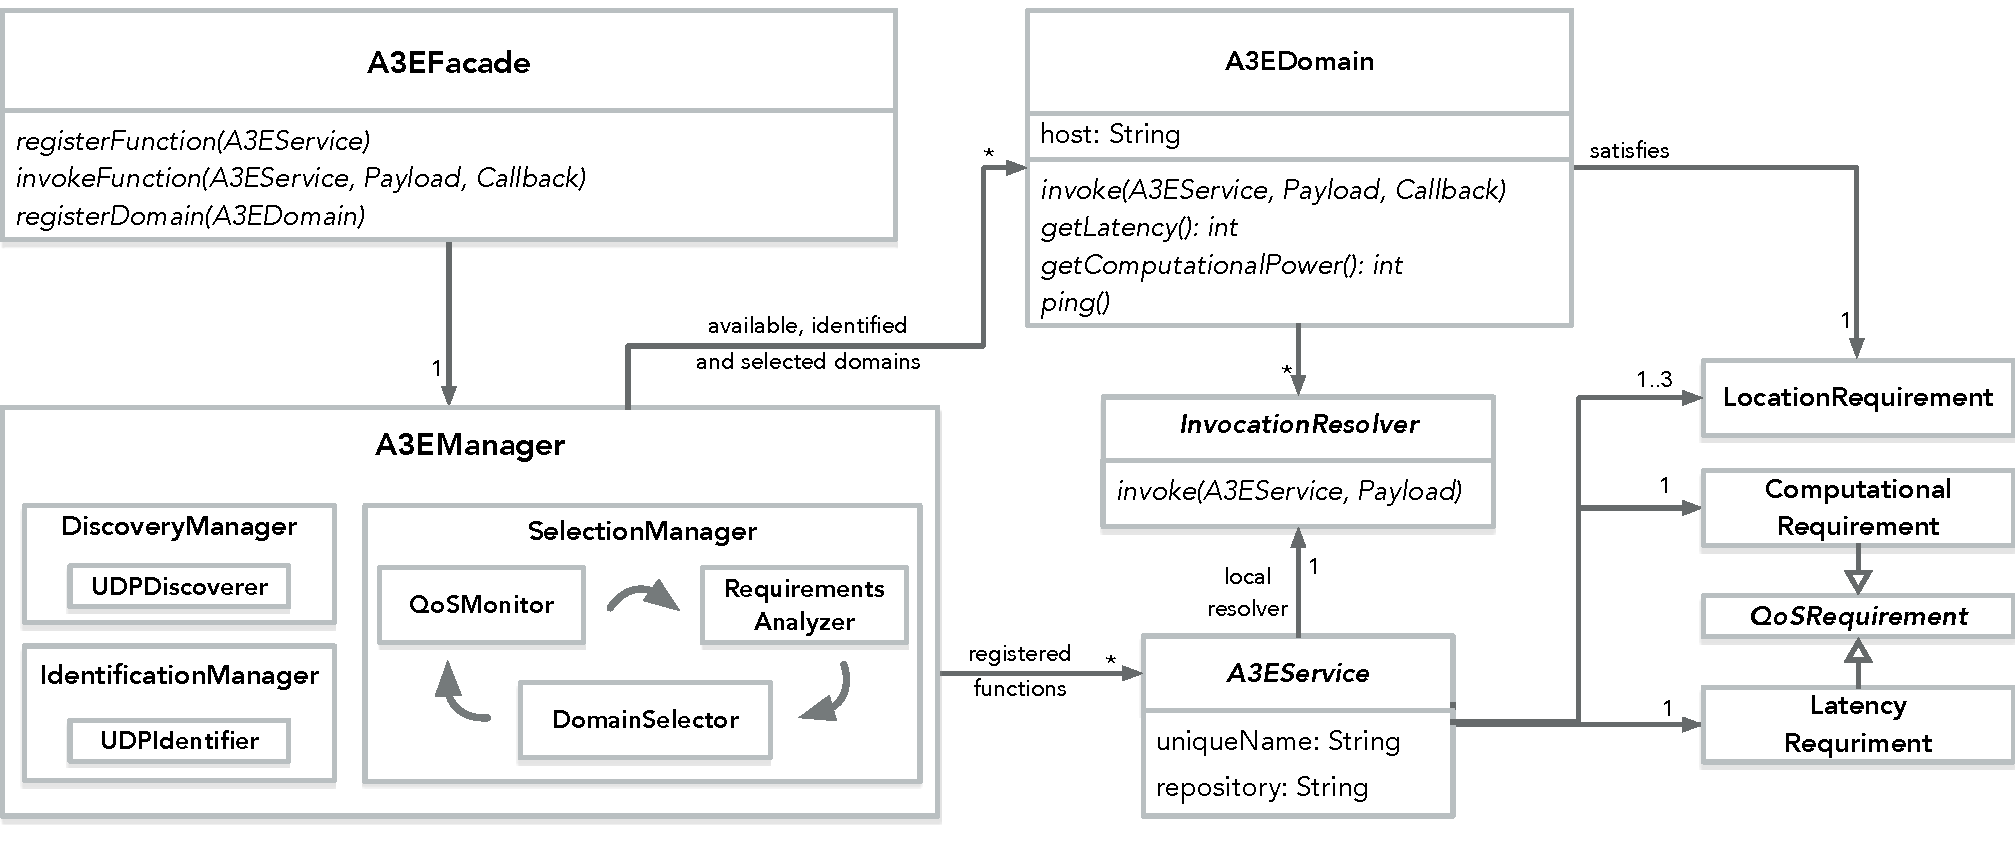
\includegraphics[width=0.9\textwidth]{figs/a3e-mobile-prototype}
	\caption{Mobile Middleware Architecture}
	\label{fig:mobile-prototype}
\end{figure}
Figure~\ref{fig:mobile-prototype} shows the architecture of the client middleware using an UML-like notation. Client mobile applications can support the continuum by simply interacting with two components:  \textit{A3EFunction}s and \textit{A3EFacade}. The former abstracts the actual functions to be executed, while the latter is the main interface by which it is possible to first register and then execute functions. An \textit{A3EFunction} is identified by a unique name that corresponds to the name of the function asset that must be communicated to the continuum domains to be first acquired and then executed. Moreover each function must declared with a set of non-functional QoS requirements that are organized in three types: 

\begin{itemize}
	\item \textit{Location Requirement}s are constrains over the continuum. A function can declare where the function could be executed choosing a combination of three values: \textit{LOCAL}, \textit{EDGE} and \textit{CLOUD}. By default an \textit{A3EFunction} supports all three domain types but one can implement one that, for example, cannot be executed locally thus only the \textit{EDGE} and \textit{CLOUD} requirements should be added to the function.    
	\item \textit{Latency Requirement} expresses how important for a function is to have a low networking latency. The default value is \textit{LOW} since the main motivation of the work is to support low-latency applications. A \textit{A3EFunction}  can be also state that this requirements should \textit{ANY} or \textit{VERY LOW}. The lower latency is requested as requirement the more the networking latency will be considered important in the the domain selection procedure.
	\item \textit{Computational Requirement} defines how relevant for a function is to have a fast computing processing. The predefined value is \textit{FAST} since, again, the main target of the approach are applications that requires fast request/response interactions. Similarly to the latency requirement two additional values are available:  \textit{ANY} or \textit{VERY FAST}. The higher  processing power is requested the more this metric will be considered important during the domain selection phase.
\end{itemize}

An \textit{A3EFunction} that support the \textit{LOCAL} location requirement should also define a local \textit{InvocationResolver}. As we are going to discuss later in this section, invocation resolvers deal with the invocation technology \textit{heterogenity}  of the continuum. For what regards the local domain we currently support the execution of native Java code and Javascript functions (that could be imported in the project as standard \textit{.js} files). For this purpose we created two \textit{InvocationResolver}s that can execute respectively Java or Javascript functions if the local domain is selected. 

The \textit{A3EFacade} wraps the \textit{A3ELoopManager} the manage a MAPE-insipired control loop for the discovery, identification and selection of domains corresponding to the \textit{Awareness}, \textit{Acquisition}, and \textit{Allocation} phases of the A3E model. The loop manager is consists of three main components called \textit{DiscoveryManager}, \textit{IdentificationManager} and \textit{SelectionManager}.

The \textit{DiscoveryManager} explores the surrounding environment looking for available domains. A domain could be \textit{static} or \textit{dynamic}. Static domains are added to the discovery manager at launch time, meaning that it is known a-priori that they will be available. Example of static domains are cloud and local ones. On contrary dynamic domains can be found only at runtime with appropriate technological protocols (such as DNS, advertising, etc.). Edge domains are not known a-priori thus they are considered dynamic. When the \textit{DiscoveryManager} find a new domain it adds to its list of available domains a new instance of  \textit{A3EDomain}. This component is identified by an \textit{host}, that is a unique identifier by which it is possible to \textit{ping} the domain. In fact, as shown in the figure, a domain is considered \textit{Pingable} that means it is possible to check for its availability and measure the networking latency to reach it.


% must be declared with two main assets: a set of requirements that states the non-functional requests of the function and a local \textit{InvocationResolver} to execute the function locally using either Java or Javascript code (described in more details later).



